\chapter{Monads}


\section{Towards Monads}
Often type constructors can be thought of as
defining \textit{``boxes''} for values, and \lstinline|Functors| with \lstinline|fmap| allow to apply functions
inside such \textit{``boxes''}.\\
\lstinline|Monad| is a constructor class introducing
operations for \textit{putting a value} into a ``box'' (\lstinline|return|) and \textit{composing} functions that return ``boxed'' values (\lstinline|bind|).\\
\textbf{``Monads"} are type constructors that are instances of \lstinline|Monad|

\note{A \textit{Type constructor} is a generic type with one or more type variables}

\subsection{\texttt{Maybe}}
\lstinline{data Maybe a = Nothing | Just a} is a type constructor with a single type variable \lstinline|a|.
A value of type \lstinline|Maybe a| is either \lstinline|Nothing| or \lstinline|Just x| for some \lstinline|x::a|.

A function \lstinline|f :: a -> Maybe b| is a partial function from
\lstinline|a| to \lstinline|b|.
\begin{lstlisting}
   father :: Person -> Maybe Person -- partial function
   mother :: Person -> Maybe Person -- (lookup in a DB)
   maternalGrandfather :: Person -> Maybe Person
   maternalGrandfather p =
   case mother p of
      Nothing -> Nothing
      Just mom -> father mom -- Nothing or a Person
\end{lstlisting}

\section{Defining Monads}


\framedt{Types and Monads}{
   What actually is a type?\\
   It may be considered a set of rules, or ``methods'' in Object-Oriented terms.
   A Monad is yet another type defined by four rules:
   \begin{itemize}
      \item bind \lstinline|>>=|
      \item then \lstinline|>>|
      \item \lstinline|return|
      \item \lstinline|fail|
   \end{itemize}
}

\note{Check out \href{http://www.idryman.org/blog/2014/01/23/yet-another-monad-tutorial/}{idryman.org/blog/2014/01/23/yet-another-monad-tutorial/}}

\newpage
\subsection{\texttt{>>=} Bind operator}

\begin{paracol}{2}
   \colfill
   \begin{lstlisting}
      class Monad m where
      (>>=) :: m a -> (a -> m b) -> m b
   \end{lstlisting}
   
   So, \lstinline|>>=| operator takes as first input a Monad containing type \lstinline|a| (a ``monadic value \lstinline|a|'') and, as second input, a first-order function taking as input \lstinline|a| and returning a Monad containing type \lstinline|b|.

   \ul{Operator is called \textbf{bind} because it binds the result
   of the left-hand action in the action on the right.}
   \colfill

   \switchcolumn
   \begin{figure}[htbp]
      \centering
      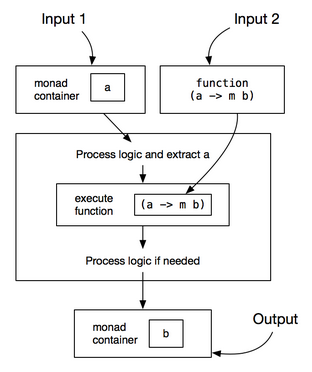
\includegraphics{images/monads_bind.png}
      \caption{Bind operator schema}
      \label{fig:monads_bind}
   \end{figure}
\end{paracol}

Hence we are introducing a higher order operator to
compose partial functions in order to
``propagate'' undefinedness automatically.

The bind operator will be part of the definition
of a monad.

\begin{lstlisting}
   y >>= g = case y of     -- y "bind" g
            Nothing -> Nothing
            Just x -> g x
\end{lstlisting}

\subsubsection{Example 1 - Grandfathers}
\begin{lstlisting}
   bothGrandfathers p =
      father p >>= 
         (\dad -> father dad >>= 
            (\gf1 -> mother p >>= 
               (\mom -> father mom >>= 
                  (\gf2 -> return (gf1, gf2)))))
\end{lstlisting}
   
\lstinline|do{}| is an alternative equivalent syntax, more \textit{imperative-like}.
\begin{lstlisting}
   bothGrandfathers p = do
      dad <- father p
      gf1 <- father dad
      mom <- mother p
      gf2 <- father mom
      return (gf1, gf2)
\end{lstlisting}

\subsubsection{Example 2 - Try catch}
\begin{lstlisting}
int errno = 0;
if (errno = io_function1( input1, &output1) == 0) {
    /* do some logic */
    if (errno = io_function2( input2, &output2) == 0) {
        /*
         * some more logic
         * and maybe more nested functions
         */
    } else {
      /* handle error 2 */
    }
} else {
    /* handle error 1 */
}

\end{lstlisting}

All the logic in this code may be represented by the Maybe monad in Haskell, where the \lstinline|Nothing| value represents any possible error.

\begin{itemize}
   \item If the first input \lstinline|M a| is \lstinline|Just x|, run the second input (the function) with value \lstinline|x|
   \item If the first input is \lstinline|Nothing|, just return \lstinline|Nothing|
\end{itemize}

When you combine several Maybe Monad handling functions together, if one of the upstream function went wrong by returning \lstinline|Nothing|, all the downstream function(s) won’t be executed

\begin{lstlisting}
   data  Maybe a  =  Nothing | Just a

   instance  Monad Maybe  where
       (Just x) >>= k      = k x
       Nothing  >>= _      = Nothing   
\end{lstlisting}

\subsubsection{Example 3 - Nested Even numbers}
\begin{lstlisting}
   maybeHalf :: Int -> Maybe Int         -- Haskell type definition
   maybeHalf a                           -- Actual function body
            | even a = Just (div a 2)
            | otherwise = Nothing


*Main> Just 10 >>= maybeHalf
Just 5
*Main> Just 10 >>= maybeHalf >>= maybeHalf
Nothing
*Main> Just 10 >>= maybeHalf >>= maybeHalf >>= maybeHalf
Nothing
            
\end{lstlisting}

User can use the defined data type Just a or Nothing to \ul{\textbf{lift} the information} (correct or error) to upper Monad.

\subsection{\texttt{>>} then operator}

The bind operator \texttt{>>=}, wraps the data and passes it to the downstream handler, but sometimes, we don't care about the wrapped value and just want to pass the state downstream. For example, performing side effects.

\begin{lstlisting}
   class Monad m where
       (>>) :: m a -> m b -> m b
       x >> y = x >>= \_ -> y   
\end{lstlisting}

Unlike bind operator \lstinline|>>=| which unwraps the value passed between user defined functions, then operator ignores the wrapped value (it uses \lstinline|_| as variable) and only captures the states \lstinline|x| and \lstinline|y|.

\begin{paracol}{2}
   
   \begin{lstlisting}
   main = putStr "What is your name?"
      >> readLn
      >>= \a -> putStr "How old are you?"
      >> readLn
      >>= \b -> print (a,b)
      
   \end{lstlisting}
   
   \switchcolumn
\begin{lstlisting}
   
   main = do putStr "What is your name?"
   a <- readLn
   putStr "How old are you?"
   b <- readLn
   print (a,b)
\end{lstlisting}
   
\end{paracol}

\subsection{\texttt{return} and \texttt{fail}}
\begin{lstlisting}
class Monad m where
   return :: a -> m a
   fail :: String -> m a 
\end{lstlisting}
The \lstinline|return| function is the wrapper that we have used so far, and \lstinline|fail| is the function to represent, as you can guess, failure. The definition of return and fail in Monad is the one above.

\lstinline|fail| can take an additional string to report the failure message. With bind, then, return, and fail functions, we then know the whole definition of the Monad type!

\begin{lstlisting}
instance  Monad Maybe  where
   (Just x) >>= k      = k x
   Nothing  >>= _      = Nothing

   (Just _) >>  k      = k
   Nothing  >>  _      = Nothing

   return              = Just
   fail _              = Nothing


\end{lstlisting}

\section{Monads as Containers and Computations}
\begin{lstlisting}
   class Monad m where -- definition of Monad type class
      return :: a -> m a
      (>>=) :: m a -> (a -> m b) -> m b -- "bind"
      (>>) :: m a -> m b -> m b -- "then"
      return :: a -> m a
      fail :: String -> m a
\end{lstlisting}
\subsection{...containers}

The monadic constructor can be seen as a container:
let’s see this for \lstinline|lists|.
{Lists in Haskell are monads because they model non-deterministic computations:\ns
\begin{itemize}
	\item A single value in the monadic context ([x]) represents a single result.
	\item A list of values in the monadic context ([x1, x2, x3]) represents multiple possible results.
\end{itemize}}
We can see that lists behave like monads by implementing the \lstinline|Monad| type class for lists, i.e. defining the \lstinline|return| and \lstinline|>>=| functions for lists.
\lstinline|return'| creates the monadic context (a list), while \lstinline|>>=-| chains computations.

\note{Note that \lstinline|List| is in fact instance of  \lstinline|Monad|}

\begin{lstlisting}
   return' :: a -> [a] -- container with single element
   return' x = [x]
   (>>=-) :: [a] -> (a -> [b]) -> [b]
   xs >>=- f = concat'(map' f xs)
   
   -- Exercise: define map and concat using bind and return
   map' :: (a -> b) -> [a] ->  [b] -- seen. "fmap" for Functors
   -- (return . f) x = return (f x) = [f x]
   map' f xs = xs >>=- (return' . f)
   concat' :: [[a]] -> [a] -- flattens two-level containers
   concat' [] = []
   concat' (xs:xss) = xs ++ concat' xss
   
   -- concat' :: Foldable t => t [a] -> [a]
   -- concat' xss = foldr (++) [] xss
\end{lstlisting}

Also \lstinline|Maybe a| is a \textit{container} for zero or one value (used for computations that might fail).
Also \lstinline|IO a| is instance of \lstinline|Monad|, and may be seen as a container for computations involving side effects: you can think of the computation as ``contained'' until it gets executed.
\lstinline|Either a b| is a container for a value \lstinline|Right b| or an error \lstinline|Left a|.
Lists instead somehow encapsulate ``multiple results'', or ``non-deterministic computations''.

\subsection{... computations}

A value of type \lstinline|m a| may be seen as a ``computation returning a value of type a''.

For any value, there is an empty computation which ``does nothing'' and
produces that result. This is given by function \lstinline|return|.

Given two computations \lstinline|x| and \lstinline|y|, one can form the computation
\lstinline|x >> y| which intuitively ``runs'' \lstinline|x|, throws away its result, then runs \lstinline|y| returning its result.

Given computation \lstinline|x|, we can use its result to decide what to do next.
Given \lstinline|f: a -> m b|, computation \lstinline|x >>= f| runs \lstinline|x|, then applies
\lstinline|f| to its result, and runs the resulting computation.

\note{Note that we can define \lstinline|then| using \lstinline|bind|:
   \lstinline|x >> y = x >>= (\_ -> y)|
}

\lstinline|return|, \lstinline|bind| and \lstinline|then| define basic ways to compose computations.
They are used in Haskell libraries to define more complex composition
operators and control structures (sequence, for-each loops, \dots).
If a type constructor defining a library of computations is monadic, one
gets automatically benefit of such libraries

Example: MAYBE
\begin{itemize}
	\item \lstinline|f:a -> Maybe b| is a partial function
	\item \lstinline|bind| applies a partial function to a possibly undefined value, propagating undefinedness
\end{itemize}
Example: LISTS
\begin{itemize}
	\item \lstinline|f:a -> [b]| is a non-deterministic function
	\item \lstinline|bind| applies a non-deterministic function to a list of values, collecting all possible results

\end{itemize}
\section{IO Monad}
\subsection{FP pros \& cons}
\labelitemize{
   \color{dkgreen}
   \textit{Pros}
}{
   \begin{itemize}
      \color{dkgreen}
      \item Concise and powerful abstractions
      \begin{itemize}
         \item higher-order functions, algebraic data types, parametric
         polymorphism, principled overloading, ...
      \end{itemize}
      \item Close correspondence with mathematics
      \begin{itemize}
         \item Semantics of a code function is the mathematical function
         \item Equational reasoning: if x = y, then f x = f y
         \item Independence of order-of-evaluation (Confluence, aka Church-Rosser)
      \end{itemize}
   \end{itemize}

   }
   \begin{figure}[htbp]
      \centering
      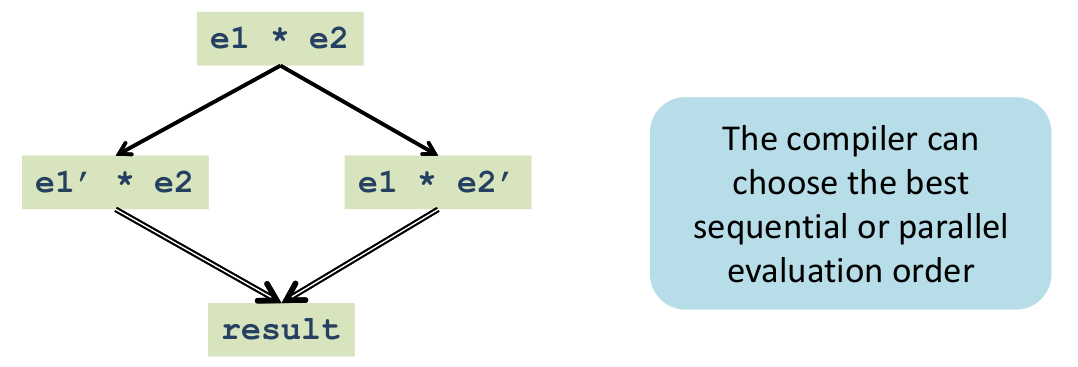
\includegraphics{images/order_eval.png}
      \caption{Evaluation order freedom}
      \label{fig:order_eval}
   \end{figure}

\labelitemize{
   \color{dkred}
   \textit{Cons}
}{
   \begin{itemize}
      \color{dkred}
      \item Input/Output
      \item Imperative update
      \item Error recovery (eg, timeout, divide by zero, etc.)
      \item Foreign-language interfaces
      \item Concurrency control
   \end{itemize}

}

Besides, recall that the whole point of a running a program is to \textbf{interact}
with the external environment and affect it

\subsection{Towards IO}
To overcome the problem of interaction, an approach is to add imperative constructs to the language,
for instance:
\begin{lstlisting}
   res = putchar 'x' + putchar 'y'
\end{lstlisting}
Seems easy right?
Well, in fact no, because \ul{in lazy languages like Haskell,
the evaluation order is \textbf{undefined}};
so, in the previous example, which char will be printed first, \lstinline|x| or \lstinline|y|?
The answer is not trivial for Haskell.
However it is not an impossible problem.
Haskell's approach is to exploit the concept of \textbf{Monads}.

Recall that the bind operator \lstinline|>>=| forces a \textbf{sequence} between the evaluation of terms;
the IO monad exploits this and defines monadic values which are called \textbf{actions}, and prescribes how to compose
them \textit{sequentially}


\subsection*{Before Monads}
Before Monads there were \textbf{Streams}, which allowed a program to send stream of requests to OS and receive stream of responses,
or the user could supply \textbf{continuations} to I/O routines
to specify how to process results.\\
However, both of these approaches revealed to be not so useful.

\subsection{Key Ideas - Monadic I/O}

\lstinline|IO| is a type constructor, instance of \lstinline|Monad|, and a value of type \lstinline|(IO t)| is an
\textit{action} (i.e. computation) that, when \textbf{performed}, may do some
input/output before delivering a result of type \lstinline|t|
\begin{itemize}
   \item 
   \lstinline|return| returns the value without making I/O
   \item
   \lstinline|then (>>)| (and also \lstinline|bind (>>=)|) composes two
   actions sequentially into a larger action
   \item
   The only way to perform an action is to call it at
   some point, directly or indirectly, from
   \lstinline|Main.main|,
   which is the standard entry point for Haskell programs.
\end{itemize}

\ul{An \textbf{action} is a \textit{first-class} value,
and \textbf{evaluating} has \textit{no effect}: \textbf{performing} the
action has the \textit{effect}}.
\note{The actual meaning of this statement is unclear even to the professor \smiley }

\begin{lstlisting}
   return :: a -> IO a
   return a = \w -> (a,w)
   (>>=) :: IO a -> (a -> IO b) -> IO b
   (>>=) m k = \w -> case m w of (r,w') -> k r w'
\end{lstlisting}
\note{\lstinline|w| \ul{is the \textit{world} (state) of the computation}}

By writing \lstinline|case m w ...| we force the evaluation of \lstinline|m|,
resulting in the application of \lstinline|k| to \lstinline|r w'| to be performed (evaluated?) \textit{after} the evaluation of \lstinline|m|.  

Let's break this a bit more:
\begin{enumerate}
	\item \lstinline{(>>=) m k}:
   This defines the bind operator \lstinline{(>>=)} for the \lstinline{IO} monad. It takes two arguments:
   \begin{itemize}
     \item \lstinline{m}: an \lstinline{IO} action that produces a value of type \lstinline{a}.
     \item \lstinline{k}: a function that takes a value of type \lstinline{a} and returns an \lstinline{IO} action producing a value of type \lstinline{b}.
   \end{itemize}
	\item \lstinline{\w -> ...}:
   This is a lambda function (anonymous function) that takes a single argument \lstinline{w}, which represents the world state.
	\item \lstinline{case m w of (r, w') -> k r w'}:
   This is a \lstinline{case} expression that evaluates the result of applying the \lstinline{IO} action \lstinline{m} to the world state \lstinline{w}.
   \begin{itemize}
     \item \lstinline{m w} produces a tuple \lstinline{(r, w')}, where \lstinline{r} is the result of the \lstinline{IO} action and \lstinline{w'} is the new world state.
     \item The \lstinline{case} expression matches this tuple and binds \lstinline{r} to the result and \lstinline{w'} to the new world state.
   \end{itemize}
	\item \lstinline{k r w'}:
   After extracting \lstinline{r} and \lstinline{w'}, the function \lstinline{k} is applied to \lstinline{r}, producing a new \lstinline{IO} action.
   This new \lstinline{IO} action is then applied to the new world state \lstinline{w'}.
\end{enumerate}

In summary, the bind operator \texttt{(>>=)} sequences two \texttt{IO} actions. It runs the first action \texttt{m}, takes its result \texttt{r}, and passes it to the function \texttt{k} to produce the next \texttt{IO} action, which is then run with the updated world state \texttt{w’}.



\subsection{\texttt{>>=} and \texttt{>>} combinators}
\ul{Operator is called \textbf{bind} because it binds the result
of the left-hand action in the action on the right.}
Performing compound action \lstinline|a >>= \x->b| :
\begin{enumerate}
   \item performs action \lstinline|a|, to yield value \lstinline|r|
   \item applies function \lstinline|\x->b| to \lstinline|r|
   \item performs the resulting action \lstinline|b{x <- r}|
   \item returns the resulting value \lstinline|v|
\end{enumerate}

\begin{figure}[htbp]
   \centering
   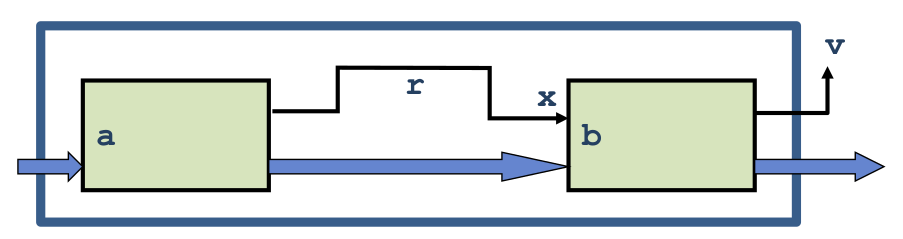
\includegraphics{images/bind_combinator.png}
   \caption{Bind Combinator}
   \label{fig:bind_combinator}
\end{figure}

The \textbf{then} combinator \lstinline|(>>)| instead does sequencing when there is no value to pass (for instance a sequence of \lstinline|putChar|s):
\begin{lstlisting}
   (>>) :: IO a -> IO b -> IO b
   m >> n = m >>= (\_ -> n)

   echoDup :: IO ()
   echoDup = getChar >>= \c ->
      putChar c >>
      putChar c
\end{lstlisting}

\subsection{\texttt{do} notation}
The ``do'' notation is a syntactic sugar for \lstinline|>>=| and \lstinline|>>|, and it is used to write monadic code in a more imperative style, making it easier to read and write.

\begin{paracol}{2}
\begin{lstlisting}
-- Do Notation
getTwoCharsDo :: IO(Char,Char)
getTwoCharsDo = do { c1 <- getChar ;
   c2 <- getChar ;
   return (c1,c2) }
\end{lstlisting}
\switchcolumn
\begin{lstlisting}
-- Plain Syntax
getTwoChars :: IO (Char,Char)
getTwoChars = getChar >>= \c1 ->
   getChar >>= \c2 ->
   return (c1,c2)
\end{lstlisting}

\end{paracol}

\begin{lstlisting}
   do { x } = x
   do { x; stmts } = x >> do { stmts }
   do { v<-x; stmts } = x >>= \v -> do { stmts }
   do {let ds; stmts } = let ds in do { stmts }
\end{lstlisting}

\subsection{Restrictions}
In pure Haskell, there is no way to transform a value of type
\lstinline|IO a| into a value of type \lstinline|a|.
\begin{lstlisting}
   unbox :: Maybe Int -> Int
   unbox (Just x) = x
   unbox Nothing  = 0   
\end{lstlisting}
While for \lstinline|Maybe| monad we can define a function \lstinline|unbox|, for \lstinline|IO| monad we cannot define a function \lstinline|unboxIO|, since the \lstinline|IO| type constructor is abstract and doesn't allow direct pattern matching of its contents in a pure function. 

Suppose you wanted to read a configuration file at the
beginning of your program:
\begin{lstlisting}
   configFileContents :: [String]
   configFileContents = lines (readFile "config") -- WRONG!
   useOptimisation :: Bool
   useOptimisation = "optimise" 'elem' configFileContents
\end{lstlisting}
The problem is that \lstinline|readFile| returns an \lstinline|IO String|, not a
\lstinline|String|.
{possible workarounds are:\ns
   \begin{enumerate}
      \item Write entire program in IO monad. But then we
      lose the simplicity of \textbf{pure} code.
      \item Escape from the IO Monad using a function from
      \lstinline|IO String -> String|. But this is \textbf{disallowed}!
   \end{enumerate}
}

We know the configuration file will \textit{not change}
during the program, so it doesn’t matter \textit{\textbf{when}} we
read it.\\
This situation arises sufficiently often that Haskell
implementations offer one last unsafe I/O primitive:
\lstinline|unsafePerformIO|
\begin{lstlisting}
   unsafePerformIO :: IO a -> a
   configFileContents :: [String]
   configFileContents = lines(unsafePerformIO(readFile "config"))
\end{lstlisting}

\ul{The operator has a deliberately long name to
\textit{discourage} its use}.
Besides, its use comes with a proof obligation:
a promise to the compiler that the \textit{timing} of this operation
relative to all other operations doesn’t matter.

It is called \textit{unsafe} because it breaks the soundness of the type system;
thus, claims that Haskell is type safe are valid only when \lstinline|unsafePerformIO| is \textbf{not} used.

\section{Summary}
\begin{itemize}
   \item A complete Haskell program is a single IO action called
   main. Inside IO, code is \textbf{single-threaded}.
   \item Big IO actions are built by gluing together smaller ones with
   \lstinline|bind (>>=)| and by converting pure code into actions with
   return.
   \item IO actions are first-class.
   They can be passed to functions, returned from functions, and
   stored in data structures; so, it is easy to define new ``glue'' combinators.
   \item The IO Monad allows Haskell to be pure while efficiently
   supporting side effects.
   \item The type system separates the \textit{pure} from the \textit{effectful} code.
\end{itemize}

\labelitemize{
   \textit{Comparison}
}{
   \begin{itemize}
      \item In languages like ML or Java, the fact that the
      language is in the IO monad is baked in to the
      language. There is no need to mark anything in the
      type system because it is everywhere.
      \item In Haskell, the programmer can choose when to live
      in the IO monad and when to live in the realm of
      pure functional programming.
      \item So it is not Haskell that lacks imperative features, but
      rather the other languages that lack the ability to
      have a statically distinguishable pure subset.
   \end{itemize}
}